\documentclass[12pt]{article}

\title{ET4340 Electronics for Quantum Computing\\Homework 4}
\author{
    Mick van Gelderen\\4091566
}
\date{November 2013}

\usepackage[utf8]{inputenc}
\usepackage[a4paper,margin=2.2cm]{geometry}
\usepackage{natbib}
\usepackage{graphicx}
\usepackage{listings}
\usepackage{framed}
\usepackage{mathtools}
\usepackage{braket}
\usepackage{ifmtarg}
\usepackage{multirow}
\usepackage{xfrac}
\usepackage{xcolor}
\usepackage{caption}
\usepackage{subcaption}
% Flat UI colors MUAHAHA

\definecolor{turquoise}{HTML}{1ABC9C}
\definecolor{emerland}{HTML}{2ECC71}
\definecolor{peter-river}{HTML}{3498DB}
\definecolor{amethyst}{HTML}{9B59B6}
\definecolor{wet-asphalt}{HTML}{34495E}
\definecolor{green-sea}{HTML}{16A085}
\definecolor{nephritis}{HTML}{27AE60}
\definecolor{belize-hole}{HTML}{2980B9}
\definecolor{wisteria}{HTML}{8E44AD}
\definecolor{midnight-blue}{HTML}{2C3E50}
\definecolor{sun-flower}{HTML}{F1C40F}
\definecolor{carrot}{HTML}{E67E22}
\definecolor{alizarin}{HTML}{E74C3C}
\definecolor{clouds}{HTML}{ECF0F1}
\definecolor{concrete}{HTML}{95A5A6}
\definecolor{orange}{HTML}{F39C12}
\definecolor{pumpkin}{HTML}{D35400}
\definecolor{pomegranate}{HTML}{C0392B}
\definecolor{silver}{HTML}{BDC3C7}
\definecolor{asbestos}{HTML}{7F8C8D}

\lstset{
        language=Matlab,                                % choose the language of the code
%       basicstyle=10pt,                                % the size of the fonts that are used for the code
        numbers=left,                                   % where to put the line-numbers
        numberstyle=\footnotesize,                      % the size of the fonts that are used for the line-numbers
        stepnumber=1,                                           % the step between two line-numbers. If it's 1 each line will be numbered
        numbersep=5pt,                                  % how far the line-numbers are from the code
        backgroundcolor=\color{clouds},          % choose the background color. You must add \usepackage{color}
        showspaces=false,                               % show spaces adding particular underscores
        showstringspaces=false,                         % underline spaces within strings
        showtabs=false,                                         % show tabs within strings adding particular underscores
%       frame=single,                                           % adds a frame around the code
        tabsize=2,                                              % sets default tabsize to 2 spaces
%       captionpos=b,                                           % sets the caption-position to bottom
        breaklines=true,                                        % sets automatic line breaking
        breakatwhitespace=false,                        % sets if automatic breaks should only happen at whitespace
        escapeinside={\%*}{*)}                          % if you want to add a comment within your code
}

\newcommand{\pauli}[1]{
    \ensuremath{
        \begin{bmatrix}
            \if#1x
                0 & 1 \\
                1 & 0 \\
            \fi\if#1y
                0 & -i \\
                i & 0 \\
            \fi\if#1z
                1 & 0 \\
                0 & -1 \\
            \fi
        \end{bmatrix}
    }
}

\setlength{\parindent}{0cm}

\newcommand{\paulisigma}[1]{%
    \ensuremath{\sigma{}_{#1}}%
}

\newcommand{\bmat}[1]{\begin{bmatrix}#1\end{bmatrix}}
\newcommand{\rsqrt}[1]{\ensuremath{\frac{1}{\sqrt{#1}}}}

\setlength{\parskip}{0.5em plus4mm minus3mm}
\newenvironment{answer}{\begingroup\setlength{\leftskip}{-\leftmargin}\begin{framed}}{\end{framed}\endgroup}

\newcommand{\CNOT}[1]{\ensuremath{\texttt{CNOT}_{#1}}}
\newcommand{\CPHASE}[1]{\ensuremath{\texttt{CPHASE}_{#1}}}
\newcommand{\SWAP}[1]{\ensuremath{\texttt{SWAP}_{#1}}}
\newcommand{\cnotgr}[1]{\ensuremath{\bmat{%
        1 & 0 & 0 & 0 \\%
        0 & 1 & 0 & 0 \\%
        0 & 0 & 0 & 1 \\%
        0 & 0 & 1 & 0 \\%
}}}

\begin{document}

\maketitle

\paragraph{Problem 1: Quantum Fourier Transform} \hfill

\begin{enumerate}

    \item Write the $8\times8$ matrix (in the computational basis) corresponding to the quantum Fourier transform on a 3-qubit register.

    \begin{answer}
        The matrix $U_{QFT,8}$ is defined as:
        \begin{align*}
            U_{QFT,8} = \rsqrt{N}\sum\limits_{l = 0}^{N - 1}\sum\limits_{k = 0}^{N - 1}e^{\frac{i2\pi{}lk}{N}}\ket{l}\bra{k}
        \end{align*}
        where $N = 8$.
        \begin{align*}\bmat{
            1 &  1 &  1 &  1 &  1 &  1 &  1 &  1 \\
            1 &  \sqrt{2} + \sqrt{2}i & i & -\sqrt{2} + \sqrt{2}i & -1 & -\sqrt{2} - \sqrt{2}i & -i &  \sqrt{2} - \sqrt{2}i \\
            1 & i & -1 & -i &  1 & i & -1 & -i \\
            1 & -\sqrt{2} + \sqrt{2}i & -i &  \sqrt{2} + \sqrt{2}i & -1 &  \sqrt{2} - \sqrt{2}i & i & -\sqrt{2} - \sqrt{2}i \\
            1 & -1 &  1 & -1 &  1 & -1 &  1 & -1 \\
            1 & -\sqrt{2} - \sqrt{2}i & i &  \sqrt{2} - \sqrt{2}i & -1 &  \sqrt{2} + \sqrt{2}i & -i & -\sqrt{2} + \sqrt{2}i \\
            1 & -i & -1 & i &  1 & -i & -1 & i \\
            1 &  \sqrt{2} - \sqrt{2}i & -i & -\sqrt{2} - \sqrt{2}i & -1 & -\sqrt{2} + \sqrt{2}i & i &  \sqrt{2} + \sqrt{2}i
        }\end{align*}
    \end{answer}

    \item Show that this matrix is unitary

    \begin{answer}
        Use a computer to calculate $U_{QFT}U_{QFT} = I$. You can easily see that the matrix is symmetric so this is the only thing we have to show.
        Matlab indeed gives $I$ with some near zero imaginary parts.
    \end{answer}

    \item Draw the quantum circuit that implements this QFT

    \begin{answer}
        From the lecture slides where it was drawn for 4 qubits:
        \begin{center}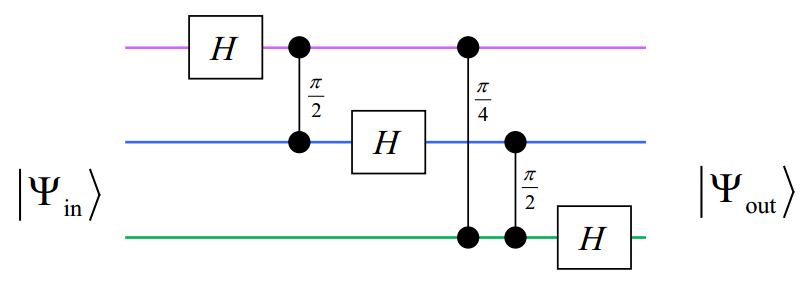
\includegraphics[width=.8\textwidth]{problem-1.png}\end{center}
    \end{answer}

\end{enumerate}

\paragraph{Problem 2: Generalized quantum kick-back} \hfill

In the lectures, we have seen how the Deutsch and Bernstein-Vazirani quantum games exploit quantum kick-back to efficiently extract properties of $n$-to-1 bit boolean functions. In this problem, we generalize quantum kick-back to $n$-to-$m$ bit boolean functions encoded in unitary functions as usual: $U_f\ket{x}\ket{y} = \ket{x}\ket{(y + f(x)) \bmod M}$ for computational states $\ket{x}$ and $\ket{y}$ in the top and bottom registers, respectively. Consider the circuit below.

\begin{center}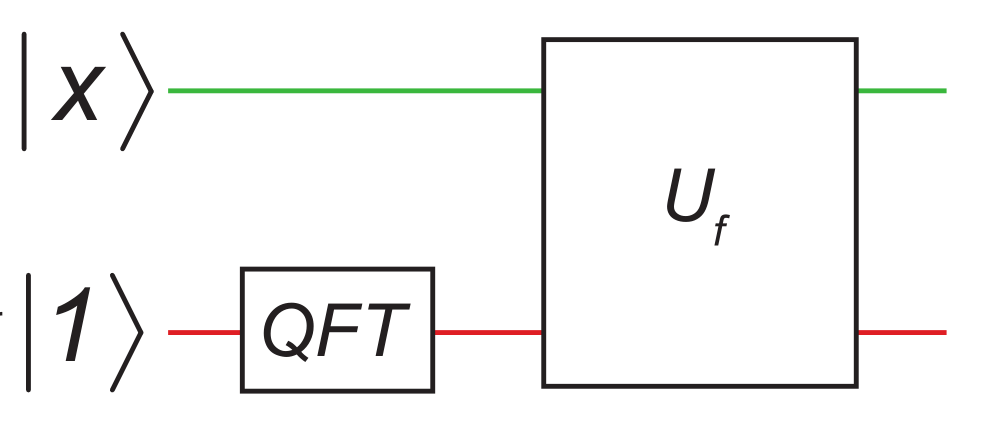
\includegraphics[width=.5\textwidth]{problem-2.png}\end{center}

\begin{enumerate}

    \item What is the state of the bottom register after application of the m-bit QFT on the initial
state $\ket{1} = \ket{00000...1}$?

    \begin{answer}
        $U_{QFT}\ket{1}$ equals the last column of $U_{QFT}$. So $U_{QFT}\ket{1} = \rsqrt{N}\sum\limits_{k = 0}^{N - 1}e^{\frac{i2\pi{}(N - 1)k}{N}}\ket{k}$
    \end{answer}

    \item Now apply $U_f$, with the top register starting in a computational state $\ket{x}$. What is the combined state of the top and bottom registers immediately after $U_f$? Show that this this state can be rewritten as:

    \begin{align*}
        e^{\frac{-i2\pi{}f(x)}{M}}\ket{x}\otimes{}U_{QFT}\ket{1},
    \end{align*}

    where $M = 2^m$. Evidently, the top and bottom registeres are not entangled, and $f(x)$ is encoded in the quantum phase of the probability amplitude!

    \begin{answer}
        The final state is:
        \begin{align*}
            \ket{x} \otimes U_f\ket{x}\ket{y} = \ket{x} \otimes \ket{x}\ket{(y + f(x)) \bmod M} \\
            \ket{x}\ket{(y + f(x)) \bmod M} = \ket{x}\ket{y} + \ket{x}\ket{f(x)} \bmod M \\
        \end{align*}
        Argh. We probably need a lecture on how to do these function encoded multi bit bullshit things, I don't have a clue how to rewrite this simply because of the notation and its angering me because I'm not able to do it.
    \end{answer}

    \item Finally, consider the case that the top register is initialized in the maximal superposition state $\rsqrt{N}(\ket{0} + \dots + \ket{N - 1})$. As usual, $N = 2^n$. What will be the final state after application of $U_f$?

    \begin{answer}
        Since $\ket{x}$ in maximal superposition is a vector of all ones, $e^{\frac{-i2\pi{}f(x)}{M}}$ is applied to all k where $0 \le k < N$. The final state is $\rsqrt{N}\sum\limits_{k = 0}^{N - 1}e^{\frac{-i2\pi{}f(k)}{M}} \otimes U_{QFT}\ket{1}$.
    \end{answer}

\end{enumerate}

\paragraph{Problem 3: Breaking RSA} \hfill

In this exercise, we will break RSA by period finding. $N$ will be small enough that we will find periods by brute force.

\begin{enumerate}
    \item List the integers $a < N$ that are co-prime with $N$. Let us pick one of these integers: let us agree to all `randomly' pick $a = 8$.

    \begin{answer}
        I guess $N = 21$.
        \begin{tabular}{c|l|l}
            $n$ & divisible by & co-primes\\
            \hline
            2 & 2 & 1 \\
            3 & 3 & 1 2 \\
            4 & 2 4 & 1 3 \\
            5 & 5 & 1 2 3 4 \\
            6 & 2 3 6 & 1 5 \\
            7 & 7 & 1 2 3 4 5 6 \\
            8 & 2 4 8 & 1 3 5 7 \\
            9 & 3 9 & 1 2 4 5 7 8 \\
            10 & 2 5 10 & 1 3 7 9 \\
            11 & 11 & 1 2 3 4 5 6 7 8 9 10 \\
            12 & 2 3 4 6 12 & 1 5 7 11 \\
            13 & 13 & 1 2 3 4 5 6 7 8 9 10 11 12 \\
            14 & 2 7 14 & 1 3 5 6 9 11 13 \\
            15 & 3 5 15 & 1 2 4 7 8 11 13 14 \\
            16 & 2 4 8 16 & 1 3 5 7 9 11 13 15 \\
            17 & 17 & 1 2 3 4 5 6 7 8 9 10 11 12 13 14 15 16 17 \\
            18 & 2 3 6 9 18 & 1 5 7 11 13 17 \\
            19 & 19 & 1 3 5 7 8 9 10 11 12 13 14 15 16 17 18 19 \\
            20 & 2 4 5 10 20 & 1 3 7 9 11 13 17 19 \\
            21 & 3 7 21 & 1 2 4 5 8 10 11 13 16 17 19 \\
        \end{tabular}
    \end{answer}

    \item Compute $8^0 \bmod 21$, $8^1 \bmod 21$, \ldots until you discover the period $r$ of $f(x) = 8^x \bmod 21$.

    \begin{answer}
        \begin{tabular}{c|c}
            $n$ & $8^n \bmod 21$ \\
            \hline
            0 & 1 \\
            1 & 8 \\
            2 & 1 \\
        \end{tabular}
        The period seems to be $2$.
    \end{answer}

    \item Find the greatest common denominator (gcd) between, $8^{\sfrac{r}{2}} + 1$ and $21$. Check whether the result is a prime factor of 21.

    \begin{answer}
        Since $r = 2$, $8^{\sfrac{r}{2}} + 1 = 9$. The gcd of $9$ and $21$ is $3$ which is indeed a prime factor of $21$.
    \end{answer}

    \item Similarly, find the gcd between $8^{\sfrac{r}{2}} - 1$ and $21$.

    \begin{answer}
        The gcd of $7$ and $21$ is $7$ which is a prime factor of $21$.
    \end{answer}

    \item Repeat the process for $a = 10$.

    \begin{answer}
        Finding the period:
        \begin{tabular}{c|c}
            $n$ & $10^n \bmod 21$ \\
            \hline
            0 & 1 \\
            1 & 10 \\
            2 & 6 \\
            3 & 13 \\
            4 & 4 \\
            5 & 19 \\
            6 & 1 \\
        \end{tabular}
        The period seems to be $6$.
        The gcd's of $10^3 \pm 1$ and $21$ are $3$ and $7$, magic!
    \end{answer}
\end{enumerate}

\paragraph{Problem 4: Breaking RSA with Shor's algorithm} \hfill

Now we will go through the steps of Shor's algorithm in order to find the period $r$ of $8^x\bmod21$. For simplicity, lest us use just four qubits for the top register which is enough for our choice of $a = 8$.
\emph{Note: Please use decimal bra-ket notation instead of binary. }

\begin{enumerate}
    \item Initialize each register to $\ket{0}$.

    \begin{answer}
    	Cool it down!
    \end{answer}

    \item Apply the hadamard gate to each qubit in the top register.

    \begin{answer}
    	The top register ends up in a state that is a combination of all possible 4 qubit computational states: $\rsqrt{16}\left(\ket{0} + \ket{1} + \dots + \ket{15}\right)$.
    \end{answer}

    \item Add $8^x\bmod21$ to the bottom register where $x$ is the state of the top register.

    \begin{answer}
    	We calculate $8^x\bmod21$ for $x \in \{0, 1, \dots 15\}$.

    	\begin{tabular}{c|c||c|c}
    		$x$ & $8^x\bmod21$ & $x$ & $8^x\bmod21$ \\
    		\hline
    		0 & 1 & 8 & 1 \\
    		1 & 8 & 9 & 8 \\
    		2 & 1 & 10 & 1 \\
    		3 & 8 & 11 & 8 \\
    		4 & 1 & 12 & 1 \\
    		5 & 8 & 13 & 8 \\
    		6 & 1 & 14 & 1 \\
    		7 & 8 & 15 & 8 \\
    	\end{tabular}

    	So, $y$ must be $\rsqrt{16}\left(\ket{1} + \ket{8} + \ket{1} + \ket{8} \dots \ket{1} + \ket{8}\right)$.
    \end{answer}

    \item Rewrite this state so you group all terms with identical $f(x)$ — observe the periodicity in the amplitudes which emerges, and observe also that you cannot efficiently reveal the period by any measurement.

    \begin{answer}
       	This means that the $y$ register is in the state $\rsqrt{2}\left(\ket{1} + \ket{8}\right)$.

       	For this simple example you might be able to measure 100 times. If you measure $\ket{1}$ 31 times and $\ket{8}$ 69 times it is probable that the period is 2 because you only measured 2 different outcomes. In general, there is a chance that if you measure $k$ times you will have not measured one or more possible outcomes which causes you to use an $r$ that is too low. For bigger N, the amount of measurements $k$ becomes very, very large to have confidence in your estimation of $r$.

       	Using the QFT is far more efficient.
    \end{answer}

    \item Apply the Quantum Fourier Transform to the top register.

    \begin{answer}
    	We apply the Quantum Fourier Transform to the top register after measurement of the bottom register.

        $U_{QFT}$ can be computed in Matlab with the following simple code:
    \end{answer}
    \lstinputlisting[language=Matlab]{../qft.m}
    \begin{answer}
        The effects of measurement can be simulated by simply only keeping the indices of the input states for which the outcome equals that measurement. This is done in the following code which also plots the state of the top register ($x$) before and after the QFT transformation.
    \end{answer}
    \lstinputlisting[language=Matlab]{code.m}
    \begin{answer}
        The above code produces the following two plots:
    \end{answer}
    \begin{figure}[h]
        \centering
        \begin{subfigure}[b]{0.45\textwidth}
                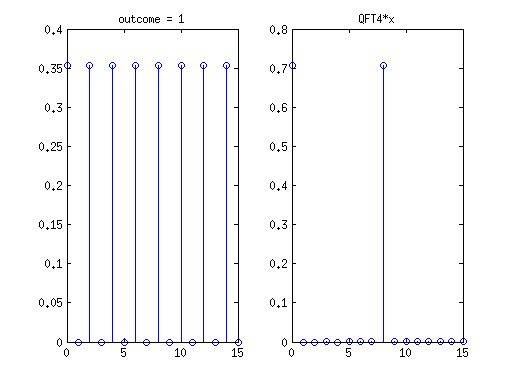
\includegraphics[width=\textwidth]{html/code_01.png}
                \caption{Measured $\ket{1}$}
                %\label{fig:gull}
        \end{subfigure}%
        ~ %add desired spacing between images, e. g. ~, \quad, \qquad etc.
          %(or a blank line to force the subfigure onto a new line)
        \begin{subfigure}[b]{0.45\textwidth}
                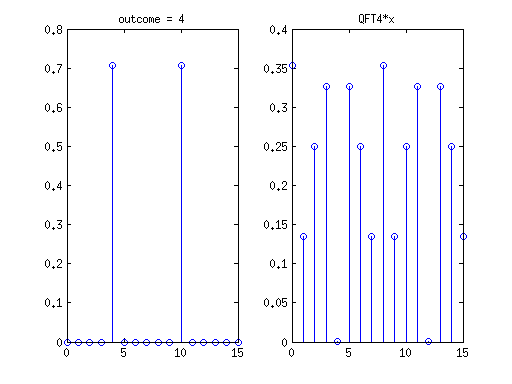
\includegraphics[width=\textwidth]{html/code_02.png}
                \caption{Measured $\ket{8}$}
                %\label{fig:tiger}
        \end{subfigure}
        \caption{Shors algorithm for $8^x\bmod21$}\label{fig:shor-plots}
    \end{figure}

    \item  Measure the final state of the top register. What are the possible measurement outcomes, and how do they relate to $r$?

    \begin{answer}
        The final states of $x$ seem to be equal when measuring both $\ket{1}$ and $\ket{8}$ for $y$. So independently of the $y$ measurement (in this case) you will have a $50\%$ chance of measuring $x = \ket{0}$ and a $50\%$ chance of measuring $x = \ket{8}$.

        If the final state of $x$ is $\ket{s}$ we can try continued fractions of prime numbers of $\frac{s}{2^{|x|}}$ and see if the denominator is a valid $r$. Obviously, when $s = 0$ you get no information about $r$.

        In our example we could measure $s = 8$ as well, this gives $8/16$. This can be simplified to $1/2$ which is a fraction of two primes. This means $r = 2$ which happens to be correct.

        After finding a possible period, we compute $\gcd(a^{\sfrac{r}{2}} \pm 1, N)$. In our case this amounts to finding $\gcd{7, 21} = 7$ and $\gcd{9, 21} = 3$. These values are primes $p$ and $q$ for which $pq = N$.
    \end{answer}

    \item  What fraction of the times that you run the algorithm above will you successfully find the factors of $21$?

    \begin{answer}
        For $a = 8$, the only final state that gives us enough information to find $p$ and $q$ is $\ket{8}$. This state occurs $50\%$ of the time.
    \end{answer}

    \item What complication occurs for $a = 10$? Discuss how Shor deals with it. \emph{Please answer this question in just a few sentences.}

    \begin{answer}
        For $a = 10$ the QFT introduces a lot of leakage. This lowers the chance of finding an $s$ that is of use in finding $r$. Shor simply suggests to run the algorithm multiple times until you find a better $s$.
    \end{answer}
\end{enumerate}

\paragraph{Problem 5: (EXTRA CREDIT) Tensor product matrices and product states} \hfill

A general tensor product of two one qubit unitaries $A$ and $B$ is given by:
\begin{align*}
    U = A \otimes B = \bmat{
        A_{11}\bmat{B_{11} & B_{12} \\ B_{21} & B_{22}} &
        A_{12}\bmat{B_{11} & B_{12} \\ B_{21} & B_{22}} \\
        A_{21}\bmat{B_{11} & B_{12} \\ B_{21} & B_{22}} &
        A_{22}\bmat{B_{11} & B_{12} \\ B_{21} & B_{22}} \\
    }
\end{align*}
\begin{enumerate}
    \item Show that a matrix of this form always takes product states to product states.

    \begin{answer}
        This property may be intuitive to you or it may not, the proof is actually not that hard.

        Lets first write $U$ a little simpler:
        \begin{align*}
            U = A \otimes B &= \bmat{
                A_{11}B &
                A_{12}B \\
                A_{21}B &
                A_{22}B \\
            }
        \end{align*}
        A product state can always be written as $\ket{\psi}\otimes\ket{\phi}$. Since vectors are essentially matrices where at least one of the dimensions is $1$, the tensor product can also be written in expanded form:
        \begin{align*}
            \ket{\psi}\otimes\ket{\phi} &= \bmat{\psi_1\ket{\phi} \\ \psi_2\ket{\phi}}
        \end{align*}
        If we can show that $U\ket{\psi}\otimes\ket{\phi} = A\ket{\psi} \otimes B\ket{\phi}$ (assuming the $\otimes$ operation is applied before the matrix product operation) we will have proven that the result of the application of the matrix $U$ can still be expressed as a product state.
        \begin{align*}
            A \otimes B\ket{\psi}\otimes\ket{\phi} &= \bmat{
                A_{11}B &
                A_{12}B \\
                A_{21}B &
                A_{22}B \\
            }\bmat{\psi_1\ket{\phi} \\ \psi_2\ket{\phi}} \\
            &=\bmat{
                A_{11}\psi_1B\ket{\phi} &
                A_{12}\psi_1B\ket{\phi} \\
                A_{21}\psi_2B\ket{\phi} &
                A_{22}\psi_2B\ket{\phi} \\
            } \\
            &=\bmat{
                A_{11}\psi_1 &
                A_{12}\psi_1 \\
                A_{21}\psi_2 &
                A_{22}\psi_2 \\
            } \otimes B\ket{\phi} \\
            &=A\ket{\psi} \otimes B\ket{\phi}
        \end{align*}
        Instead of a mathmatical proof, we can simply look at the way the quantum circuit is represented. $U$ is essentially a two-qubit gate composed of two single qubit gates $A$ and $B$. This means that it is impossible for the two qubits to interact which in turn means that they cannot become entangled. Since entanglement is required to prevent two qubits from being written as a product state, $U$ cannot possibly prevent the outcome from being written as a product state.
    \end{answer}

    \item Prove that the \CNOT{} gate cannot be written in this form by comparing the matrix entries with the general tensor product matrix above.

    \begin{answer}
        The transformation matrix for the two qubit \CNOT{} is:
        \begin{align*}
            \CNOT{} = \bmat{
                1 & 0 & 0 & 0 \\
                0 & 1 & 0 & 0 \\
                0 & 0 & 0 & 1 \\
                0 & 0 & 1 & 0 \\
            }
        \end{align*}
        Lets define $A$ and $B$ as follows:
        \begin{align*}
            A &= \bmat{a & b \\ c & d} \\
            B &= \bmat{w & x \\ y & z}
        \end{align*}
        From the entire matrix multiplication we can deduce the following contradicting equations:
        \begin{align*}
            aw &= 1 & ax &= 0 \\
            dw &= 0 & dx &= 1
        \end{align*}
        Because $ax = 0$ we must set either $a$ or $x$ to 0. In case we pick $a$, it becomes impossible to pick $w$ so that $aw = 0w = 1$. In case we pick $x$ it becomes impossible to find a $d$ so that $dx = d0 = 1$.

        This means that it is impossible to construct \CNOT{} from $A \otimes B$.

        This is only natural since the \CNOT{} operation requires a qubit to flip depending on the state of the other. In other words, they must interact. This is impossible with two single qubit gates.
    \end{answer}

    \item Show that the \SWAP{} gate always takes a product state to another product state.

    \begin{answer}
        The transformation matrix for \SWAP{} is:
        \begin{align*}
            \SWAP{} = \bmat{
                1 & 0 & 0 & 0 \\
                0 & 0 & 1 & 0 \\
                0 & 1 & 0 & 0 \\
                0 & 0 & 0 & 1 \\
            }
        \end{align*}
        Writing out a product state as a vector and applying \SWAP{} yields:
        \begin{align*}
            \ket{\psi}\otimes\ket{\phi} &= \bmat{
                \psi_1\phi_1 \\
                \psi_1\phi_2 \\
                \psi_2\phi_1 \\
                \psi_2\phi_2
            } \\
            \SWAP{}\ket{\psi}\otimes\ket{\phi} &= \bmat{
                \psi_1\phi_1 \\
                \psi_2\phi_1 \\
                \psi_1\phi_2 \\
                \psi_2\phi_2
            } = \ket{\phi}\otimes\ket{\psi}
        \end{align*}
    \end{answer}

    \item Can you write the \SWAP{} gate in the form of $A \otimes B$? If so give your solution for $A$ and $B$. If not give a proof.

    \begin{answer}
        The proof for this is similar to that of the \CNOT{}. This time you have:
        \begin{align*}
            aw &= 1 & ax = 0 \\
            cw &= 0 & cx = 1
        \end{align*}
        These equations are also inconsistent.

        This is a counter example to the statement `if a two cubit gate cannot be expressed in single cubit gates, the result of applying the gate to a product state will not yield a product state'.
    \end{answer}
\end{enumerate}
\end{document}

